


%============================================================================%
%
%	DOCUMENT DEFINITION
%
%============================================================================%

%we use article class because we want to fully customize the page and dont use a cv template
\documentclass[10pt,A4]{article}	


%----------------------------------------------------------------------------------------
%	ENCODING
%----------------------------------------------------------------------------------------

%we use utf8 since we want to build from any machine
\usepackage[utf8]{inputenc}		

%----------------------------------------------------------------------------------------
%	LOGIC
%----------------------------------------------------------------------------------------

% provides \isempty test
\usepackage{xifthen}

%----------------------------------------------------------------------------------------
%	FONT
%----------------------------------------------------------------------------------------

% some tex-live fonts - choose your own

%\usepackage[defaultsans]{droidsans}
%\usepackage[default]{comfortaa}
%\usepackage{cmbright}
\usepackage[default]{raleway}
%\usepackage{fetamont}
%\usepackage[default]{gillius}
%\usepackage[light,math]{iwona}
%\usepackage[thin]{roboto} 
\usepackage{hyperref}
% set font default
\renewcommand*\familydefault{\sfdefault} 	
\usepackage[T1]{fontenc}

% more font size definitions
\usepackage{moresize}		


%----------------------------------------------------------------------------------------
%	PAGE LAYOUT  DEFINITIONS
%----------------------------------------------------------------------------------------

%debug page outer frames
%\usepackage{showframe}			


%define page styles using geometry
\usepackage[a4paper]{geometry}		

% for example, change the margins to 2 inches all round
\geometry{top=1.25cm, bottom=-.6cm, left=1.5cm, right=1.5cm} 	

%use customized header
\usepackage{fancyhdr}				
\pagestyle{fancy}

%less space between header and content
\setlength{\headheight}{-5pt}		


%customize entries left, center and right
%\lhead{}
%\chead{}
%\rhead{}


%indentation is zero
\setlength{\parindent}{0mm}

%----------------------------------------------------------------------------------------
%	TABLE /ARRAY DEFINITIONS
%---------------------------------------------------------------------------------------- 

%for layouting tables
\usepackage{multicol}			
\usepackage{multirow}

%extended aligning of tabular cells
\usepackage{array}

\newcolumntype{x}[1]{%
>{\raggedleft\hspace{0pt}}p{#1}}%


%----------------------------------------------------------------------------------------
%	GRAPHICS DEFINITIONS
%---------------------------------------------------------------------------------------- 

%for header image
\usepackage{graphicx}

%for floating figures
\usepackage{wrapfig}
\usepackage{float}
%\floatstyle{boxed} 
%\restylefloat{figure}

%for drawing graphics		
\usepackage{tikz}				
\usetikzlibrary{shapes, backgrounds,mindmap, trees}


%----------------------------------------------------------------------------------------
%	Color DEFINITIONS
%---------------------------------------------------------------------------------------- 

\usepackage{color}

%accent color
\definecolor{sectcol}{RGB}{0,150,255}

%dark background color
\definecolor{bgcol}{RGB}{110,110,110}

%light background / accent color
\definecolor{softcol}{RGB}{225,225,225}


%============================================================================%
%
%
%	DEFINITIONS
%
%
%============================================================================%

%----------------------------------------------------------------------------------------
% 	HEADER
%----------------------------------------------------------------------------------------

% remove top header line
\renewcommand{\headrulewidth}{0pt} 

%remove botttom header line
\renewcommand{\footrulewidth}{0pt}	  	

%remove pagenum
\renewcommand{\thepage}{}	

%remove section num		
\renewcommand{\thesection}{}			

%----------------------------------------------------------------------------------------
% 	ARROW GRAPHICS in Tikz
%----------------------------------------------------------------------------------------

% a six pointed arrow poiting to the left
\newcommand{\tzlarrow}{(0,0) -- (0.2,0) -- (0.3,0.2) -- (0.2,0.4) -- (0,0.4) -- (0.1,0.2) -- cycle;}	

% include the left arrow into a tikz picture
% param1: fill color
%
\newcommand{\larrow}[1]
{\begin{tikzpicture}[scale=0.58]
	 \filldraw[fill=#1!100,draw=#1!100!black]  \tzlarrow
 \end{tikzpicture}
}

% a six pointed arrow poiting to the right
\newcommand{\tzrarrow}{ (0,0.2) -- (0.1,0) -- (0.3,0) -- (0.2,0.2) -- (0.3,0.4) -- (0.1,0.4) -- cycle;}

% include the right arrow into a tikz picture
% param1: fill color
%
\newcommand{\rarrow}
{\begin{tikzpicture}[scale=0.7]
	\filldraw[fill=sectcol!100,draw=sectcol!100!black] \tzrarrow
 \end{tikzpicture}
}



%----------------------------------------------------------------------------------------
%	custom sections
%----------------------------------------------------------------------------------------

% create a coloured box with arrow and title as cv section headline
% param 1: section title
%
\newcommand{\cvsection}[1]
{
	\begin{center}
		\large\textcolor{sectcol}{\textbf{#1}}
	\end{center}
}

%create a coloured arrow with title as cv meta section section
% param 1: meta section title
%
\newcommand{\metasection}[2]
{
%\begin{tabular*}{1\textwidth}{r r}
\footnotesize{#2} \hspace*{\fill} \footnotesize{#1}\\[1pt]
%\end{tabular*}
}

%----------------------------------------------------------------------------------------
%	 CV EVENT
%----------------------------------------------------------------------------------------

% creates a stretched box as cv entry headline followed by two paragraphs about 
% the work you did
% param 1:	event time i.e. 2014 or 2011-2014 etc.
% param 2:	event name (what did you do?)
% param 3:	institution (where did you work / study)
% param 4:	what was your position
% param 5:	some words about your contributions
% param 6: moree contributions

\newcommand{\cvevent}[6]
{

\begin{tabular*}{1\textwidth}{p{13.6cm}  x{3.9cm}}
	\textbf{#2} - \textcolor{bgcol}{#3} &   \vspace{2.5pt}\textcolor{sectcol}{#1}
\end{tabular*}

\vspace{-11pt}
\textcolor{softcol}{\hrule}
\vspace{3pt}

  $\cdot$ #4\\[3pt]
  $\cdot$ #5\\[6pt]
  $\cdot$ #6\\[6pt]

}
\newcommand{\cvevent}[5]
{

\begin{tabular*}{1\textwidth}{p{13.6cm}  x{3.9cm}}
	\textbf{#2} - \textcolor{bgcol}{#3} &   \vspace{2.5pt}\textcolor{sectcol}{#1}
\end{tabular*}

\vspace{-11pt}
\textcolor{softcol}{\hrule}
\vspace{3pt}

  $\cdot$ #4\\[3pt]
  $\cdot$ #5\\[6pt]
  $\cdot$ #6\\[6pt]

}

% creates a stretched box as 
\newcommand{\cveventmeta}[2]
{
	\mbox{\mystrut \hspace{87pt}\textit{#1}}\\
	#2
}

%----------------------------------------------------------------------------------------
% CUSTOM STRUT FOR EMPTY BOXES
%----------------------------------------- -----------------------------------------------
\newcommand{\mystrut}{\rule[-.3\baselineskip]{0pt}{\baselineskip}}

%----------------------------------------------------------------------------------------
% CUSTOM LOREM IPSUM
%----------------------------------------------------------------------------------------
\newcommand{\lorem}
{Lorem ipsum dolor sit amet, consectetur adipiscing elit. Donec a diam lectus.}



%============================================================================%
%
%
%
%	DOCUMENT CONTENT
%
%
%
%============================================================================%
\begin{document}


%use our custom fancy header definitions
\pagestyle{fancy}	





%----------------------------------------------------------------------------------------
%	HEADER IMAGE
%----------------------------------------------------------------------------------------

%\begin{figure}[H]
%\begin{flushright}
%	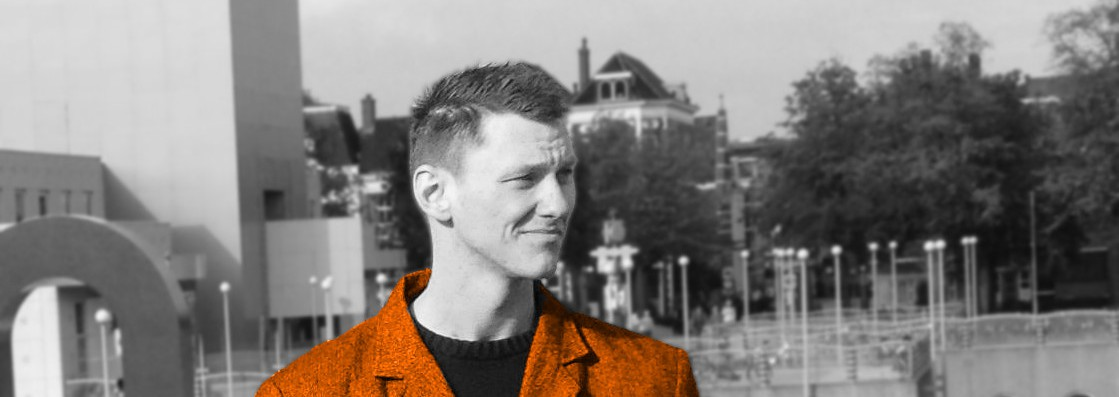
\includegraphics[trim= 320 130 460 210,clip,width=0.2\linewidth]{myfoto.jpg}	%trimming relative to image size!
%\end{flushright}
%\end{figure}


%---------------------------------------------------------------------------------------
%	TITLE HEADLINE
%----------------------------------------------------------------------------------------
\vspace{-8pt}
\begin{center}
	\HUGE \textsc{Tikam Alma} \textcolor{sectcol}{\rule[-1mm]{1mm}{0.9cm}} \textsc{Resume}\\[2pt]
	\small FullStack Developer | Security Developer 
\end{center}



\vspace{6pt}


%---------------------------------------------------------------------------------------
%	META SECTION
%----------------------------------------------------------------------------------------
\metasection{\href{https://www.linkedin.com/in/tikam-alma-993225b8/}{Linkedin}}{\textbf{Status:} B.tech, IT and ICT, DAIICT Gandhinagar}
\metasection{\href{https://github.com/Tikam02}{https://github.com/Tikam02}}{\textbf{Fields:} Full-Stack Web Devlopment, Security Development, Bug-Bounty Hunting, Machine Learning} 
\metasection{\href{tikamalma1@gmail.com}{tikamalma1@gmail.com}}{\textbf{Prefers:} JS, Python, Node.js, React.js, Django, C/C++, Linux, Git,}
\metasection{+91 8154940247}{\textbf{Activities:} OWASP Project Developer, Bughiest Site Engineer, Security+ML Research, Portrait Artist}
\vspace{-2pt}
\textcolor{softcol}{\hrule}
\vspace{6pt}

\normalsize

%---------------------------------------------------------------------------------------
%	SUMMARAY (optional)
%----------------------------------------------------------------------------------------
\vspace{-6pt}
\cvsection{Summary}
Undergraduate student at DAIICT-Gandhinagar, Bachelors Degree:ICT.
Currently working on open-source projects of Open Web Application Security projects and frameworks.Machine Learning enthusiast,learning and implementing.Researching on topics of Cyber Security and machine learning to blend it.\\


%============================================================================%
%
%	CV SECTIONS AND EVENTS (MAIN CONTENT)
%
%============================================================================%

%---------------------------------------------------------------------------------------
%	EXPERIENCE
%----------------------------------------------------------------------------------------
\cvsection{Experience}

%
\cvevent{May 2018 - July 2018}{Machine Learning-Engineer Internship}{http://infiniumsolutionz.com}{Implemented Crowd Estimation technology through Deep Learning Approach.}{Implemented and Experimented various research papers to get optimized result.}{Learnt and Implemented the project via CNN,FCNN,MCNN,CrowdNet and Frameworks:Tensorflow,Keras,Pytorch.}

%\textcolor{softcol}{\hrule}

%
\cvevent{December 2017}{Rural Internship}{http://hifeed.org/}{Exposure to the rural villages and solved their problems.}{Built a forum and communication website for self-help Woman's community for their easy communication and spreading awareness.}{Worked,survey and implemented solutions to the problems of vocational and educational training in rural areas.}

%\textcolor{softcol}{\hrule}


%
\cvevent{June 2017 - August2017}{Security Developer Intern}{https://www.owasp.org}{Selected as and intern for open web application security- Offensive Web Testing Framework(OWTF-Project)}{Implemented SSH testing and network protocols.}{Framework vulnerability testing and Django UI/UX implementation}


%---------------------------------------------------------------------------------------
%	PROJECTS
%----------------------------------------------------------------------------------------
\cvsection{Projects}

%
\cvevent{May 2018-Present}{Network Security+ML}{https://github.com/Tikam02/MLSec}{ML based network and Packet Analyzer}{Technologoy  used:Tensorflow+Pandas+Numpy+Scikit+Wireshark+Snort.}{Purpose:To learn network and packet analysis through machine learning}

%\textcolor{softcol}{\hrule}

%
\cvevent{Mar 2018-May 2018}{Top Trends}{https://github.com/Tikam02/Top-Trends}{Top-Trends is Python+Django based Fullstack internet web crawler that crawls through site and updates trending stories and articles }{Technology:Python+Scipy+Scikit+Pandas+Numpy+Bootstrap}{Purpose:To implement a full stack rest framework with crawler.}

%\textcolor{softcol}{\hrule}

%
\cvevent{Jan 2018-Feb 2018}{Wine Shop}{https://github.com/Tikam02/Wine-Shop}{Machine Learning based  recommendation engine using K-means clustering algorithm.}{Tech Used:Python+Django+bootstrap.}
{Purpose:Learning and implementation of basic ML algorithms.}


%---------------------------------------------------------------------------------------
%	EDUCATION SECTION
%--------------------------------------------------------------------------------------
\cvsection{Education}

\cvevent{2016-2020}{}{DAIICT-Gandhinagar}{Undergraduate Student:ICT}{Developer student Community}{Activities:Basketball,Portrait Sketching,Books}




%--------------------------------------------------------------------------------------------------
%	ARTIFICIAL FOOTER (fancy footer cannot exceed linewidth) 
%--------------------------------------------------------------------------------------------------

\null
\vspace*{\fill}
\hspace{-0.25\linewidth}\colorbox{bgcol}{\makebox[1.5\linewidth][c]{\mystrut \small \textcolor{white}{\href{https://www.linkedin.com/in/tikam-alma-993225b8/}{Linkedin}} $\cdot$ \textcolor{white}{\href{https://github.com/Tikam02}{Github}}}}





%============================================================================%
%
%
%
%	DOCUMENT END
%
%
%
%============================================================================%
\end{document}

